\documentclass[utf8x]{beamer} 
\renewcommand{\figurename}{圖}
\usepackage[boldfont,slantfont,CJKnumber,CJKaddspaces]{xeCJK}
\setCJKmainfont{BiauKai}

\usepackage{fontspec} %加這個就可以設定字體 
\usepackage{pstricks,pst-node,pst-tree}
\usepackage{fancyvrb}
\usepackage{xcolor}
\usepackage{marvosym}
%\usepackage{enumitem}

\XeTeXlinebreaklocale "zh" 
\XeTeXlinebreakskip = 0pt plus 1pt

\useoutertheme{infolines}
\usetheme{Singapore}%{PaloAlto}%{PaloAlto} %{Berkeley}

\usecolortheme[RGB={107,142,35}]{structure}
\setbeamertemplate{navigation symbols}{}
\setbeamertemplate{blocks}[rounded][shadow=false]
\logo{\includegraphics[height=0.8cm]{logo.pdf}}
%\setbeamertemplate{background canvas}{
%\begin{picture}(364,300)(0,0)
%\put(0,250){%(308,225){%
%  \parbox[b]{50cm}{
%     \includegraphics[width=1.8cm,keepaspectratio]{logo.pdf}
%    }
%   }
%\end{picture}

%}

\begin{document} 
\date[7/8/2011]{7/8/2011 TCSE-2011 報告} 
\title[跨平台軟體持續整合樣式之已知案例探討]{跨平台軟體持續整合樣式之\\已知案例探討} 
\author[王熙鈞] 
        { 王熙鈞\inst{} \and 鄭有進\inst{\ddag} \and 謝金雲\inst{\ddag} \and 陳建村\inst{\ddag} } 
\institute[國立臺北科技大學資訊工程系] 
        {   \inst{\ddag}共同作者 } 




\begin{frame}%---------title page 
    \titlepage\end{frame} 


\begin{frame}%---------outline page 

\frametitle{Outline} 

\begin{itemize}
\setlength{\itemindent}{1em}
\item 背景介紹\hspace{3pt}-\hspace{3pt}跨平台軟體\hspace{2pt}\textbf{持續整合}\ddag\hspace{2pt}樣式\dag
%\item[] 研究目的
%\begin{itemize}
\item 探討Project範疇樣式語言已知案例%\hspace{3pt}-\hspace{3pt}slide 7$\sim$15
%\item 探討Build範疇樣式語言已知案例並演化之%\hspace{3pt}-\hspace{3pt}slide 16$\sim$19
%\end{itemize}
%\item 探討Good Habit範疇樣式語言已知案例並演化之
\item 結論%\hspace{3pt}-\hspace{3pt}slide 20
\fontsize{6pt}{4pt}\selectfont
\item[] $\ddag$Martin Fowler's articel about Continuous Integation [online]. Available:http:// martinfowler.com/articles/originalContinuousIntegration.html.
\item[] $\dag$Chin-Yun Hsieh, Yu Chin Cheng, and Chien-Tsun Chen. \\Emerging patterns of continuous integration for cross-platform software development. In AsianPLoP, 2011.
\end{itemize}
\end{frame} 
 
 %\begin{frame}%---------背景介紹 outline page 

%\frametitle{背景介紹 Outline} 

%\begin{enumerate}
%\item 跨平台軟體開發
%\item 持續整合
%\item 樣式與樣式語言
%\item 跨平台軟體持續整合樣式語言
%\item 於Portland Pattern Repository發表的持續整合樣式
%\end{enumerate} 
         
 %\end{frame} 


%\begin{frame}%---------跨平台軟體開發 page 
%\frametitle{跨平台軟體開發}
%\begin{enumerate}
%\item 特性
%\begin{enumerate}
%\item 相依同一份原始碼進行開發
%\item 同一釋出版本中包含相容不同平台之產品
%\item 匯集於不同平台上開發軟體之工程師%、擁有不同開發程式之次文化、來自不同地區。
%\end{enumerate}
%\item 挑戰
%\begin{enumerate}
%\item 設計面
%\item 需求面
%\item 流程面
%\end{enumerate}
%\end{enumerate}
%\end{frame} 

%\item 為什麼要開發跨平台軟體
%\begin{enumerate}
%\item 商業策略%---------Market share
%有很多其他的作法,why bother.
%
%\item 比較跨平台軟體開發與移植
%\end{enumerate}

%\item 高難度開發技術
%\begin{enumerate}
%\item 抽象化各個平台的特性
%\item 與平台有關的程式碼需要被侷限
%\item 測試成本數倍於單一平台測試
%\end{enumerate}

%\begin{frame}
%\frametitle{開發跨平台軟體的挑戰\hspace{3pt}-\hspace{3pt}設計面}
%\begin{enumerate}%1
%\item 如何提供抽象化介面
%\item 抽象化介面如何運作
%\begin{enumerate}%2
%\item 封裝與平台相關的程式碼
%\item 與平台無關的程式碼只與介面相依
%\item 與平台相關之實作依循介面實作 
%\end{enumerate}%2
%\item 好處
%\begin{enumerate}%2
%\item 便利不同平台之開發者分工進行實作%實作功能僅需相依與平台有關之程式碼
%\item 避免開發者同時對同一檔案進行修改而發生衝突%不同平台之開發者相依同一檔案進行實作
%\end{enumerate}%2
%\end{enumerate}%1
%\end{enumerate}
%\end{frame}

%\begin{frame}
%\frametitle{開發跨平台軟體的挑戰\hspace{3pt}-\hspace{3pt}需求面}
%\begin{enumerate}
%\item 相同需求於不同平台實現的難易程度不一致
%\begin{enumerate}
%\item 於iOS, Android平台利用HTTPS存取網頁。
%\end{enumerate}
%\item 功能無法以最佳效能呈現
%\begin{enumerate}
%\item 多媒體播放軟體利用GPU加速
%\item 相依於Windows平台專用API
%\item 顧及相依共同介面
%\item 需放棄
%\end{enumerate}
%\end{enumerate}
%\end{frame}

%\begin{frame}
%\frametitle{開發跨平台軟體的挑戰\hspace{3pt}-\hspace{3pt}流程面}
%\begin{enumerate}
%\item 於為數眾多的平台上進行測試造成成本上升\hspace{3pt}-\hspace{3pt}必須自動化執行以降低成本
%\item 開發者撰寫適用於特定平台的程式碼而造成軟體無法在其他平台建置\hspace{3pt}-\hspace{3pt}必須實踐跨平台軟體建置整合%不同平台的開發人員修改置放同一版本控制系統中的程式碼,因為撰寫適用於特定平台的程式碼而造成軟體無法在其他平台建置,該開發者在不知情的狀況下簽入版本控制系統,進而導致其他開發者無法進行開發工作。
%\end{enumerate}
%\end{frame}

%\begin{frame}%---------持續整合
%\frametitle{持續整合}
%\begin{enumerate}
%\item 特性
%\begin{enumerate}
%\item 有效減低風險\hspace{3pt}-\hspace{3pt}越早且經常執行高風險工作
%\item 永續性
%\end{enumerate}
%\end{enumerate}
%\begin{enumerate}
%\item 整合
%\begin{enumerate}
%\item 難以估計時程
%\item 高風險
%\item 通常於軟體開發末期進行
%\item 越高風險的工作應該越早、經常被執行
%\end{enumerate}
%\item 持續
%\begin{enumerate}
%\item 頻率增加\hspace{3pt}-\hspace{3pt}每次有程式碼簽入版本控制系統時,將執行一次整合工作。
%\item 永續性
%\end{enumerate}
%\item 開發軟體常見風險\hspace{3pt}-\hspace{3pt}同時適用於開發跨平台軟體
%\begin{enumerate}
%\item 缺乏可交付的軟體
%\item 缺乏找尋軟體缺陷的機制
%\item 缺乏了解軟體專案狀態的機制
%\item 低落的軟體品質
%\end{enumerate}
%\item Broken Build
%\end{enumerate}
%\end{frame}

%\begin{frame}
%\frametitle{持續整合}
%\begin{enumerate}
%\item 無法永續的原因
%\begin{enumerate}
%\item 進行持續整合會對軟體開發團隊造成衝擊
%\begin{enumerate}
%\item 測試案例量大且耗時
%\item 軟體架構未因應實踐持續整合而修改
%\end{enumerate}
%\end{enumerate}
%\item 無法只依賴工具
%\item 注重實踐經驗傳承
%\end{enumerate}
%\end{frame}

%\begin{frame}%----------樣式
%\frametitle{樣式}
%\begin{enumerate}%1
%\item 目標:特定情境下解決特定問題
%\item 產生問題之原因:互相衝突的現象
%\item 樣式如何解決問題:平衡現象
%\begin{enumerate}%2
%\item 一併平衡導入樣式而形成的衝擊
%\end{enumerate}%2
%\item 表達樣式需包含情境、現象、解法
%\item 樣式為經驗與知識之傳遞工具
%\end{enumerate}
%\end{frame}

%\begin{frame}%------樣式之間的關係
%\frametitle{樣式之間的關係}
%\begin{enumerate}
%\item 如果樣式A要解決預定要解的問題,樣式B必須替樣式A解決一部分的問題。
%\item 樣式間關係形成網絡
%\end{enumerate}
%\begin{center}
%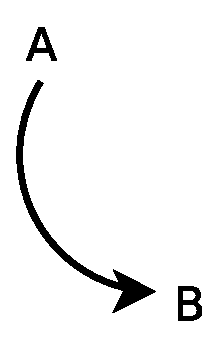
\includegraphics[width=1.5cm]{pattern-connection.eps}
%\end{center}
%\end{frame}

%\begin{frame}%--------樣式語言
%\frametitle{樣式語言}
%\begin{enumerate}
%\item 特定情境下
%\item 目標:解決問題(更為巨大)
 %\item 產生問題之原因:互相衝突的現象(為數更多)
 %\item 如果樣式A要解決預定要解的問題,\\樣式B必須替樣式A解決一部分的問題。
%\item 樣式間關係形成網絡
%\end{enumerate}
%\item 樣式網絡形成一種語言
%\begin{enumerate}
%\item 描述多個樣式如何協同合作平衡現象
%\item 傳承解決問題之經驗與知識
%\end{enumerate}
%\item 導入樣式形成的衝擊一併平衡。
%\end{enumerate}
%\begin{center}
%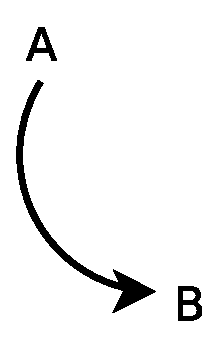
\includegraphics[width=1.5cm]{pattern-connection.eps}
%\end{center}
%\end{frame}

\begin{frame}
\frametitle{跨平台軟體持續整合樣式}
\begin{itemize}
\setlength{\itemindent}{1em}
\item[] 情境:跨平台軟體開發團隊實踐持續整合
\item[] 實踐持續整合之目的:降低開發風險
\begin{itemize}
\setlength{\itemindent}{3em}
\item[風險] 無可交付之軟體、無法掌握專案狀況、無法掌握軟體品質、軟體產品品質不佳\ddag
\end{itemize}
\item[] 樣式表達、傳承下列知識
\begin{itemize}
\item 降低開發跨平台軟體之風險(成本)
\item 克服實踐持續整合帶來的衝擊永續執行持續整合
\end{itemize}
\item[] Project, Build, Good Habit 三大範疇樣式預定達成之目的
\begin{itemize}
\item 如何依循separation of concern與module decomposition改善軟體架構\dag%Project 範疇樣式語言預定達成的目的
\item 如何避免Broken Build\dag\dag%Build 範疇樣式語言預定達成的目的
\item 如何處理Broken Build%Good Habit 範疇樣式預定達成的目的
\end{itemize}
\fontsize{6pt}{4pt}\selectfont
\item[] $\dag$$\dag$,$\ddag$Paul M. Duvall, Steve Matyas, and Andrew Glover.\\Continuous Integration: Improving Software Quality and Reducing Risk.\\Addison-Wesley Professional, 2007.
\item[] $\dag$Len Bass, Paul Clements, and Rick Kazman. Software Architecture in Practice.
\\Addison-Wesley Professional, 2003.
\end{itemize}
\end{frame}

%\begin{frame}
%\frametitle{研究目的}
%\begin{description}
%\item[] 於跨平台軟體專案實例中找尋已知案例
%\item[] 演化樣式語言
%\end{description}
%\end{frame}

\begin{frame}
\frametitle{跨平台軟體持續整合\\樣式語言 \textendash\hspace{6pt}樣式網絡}
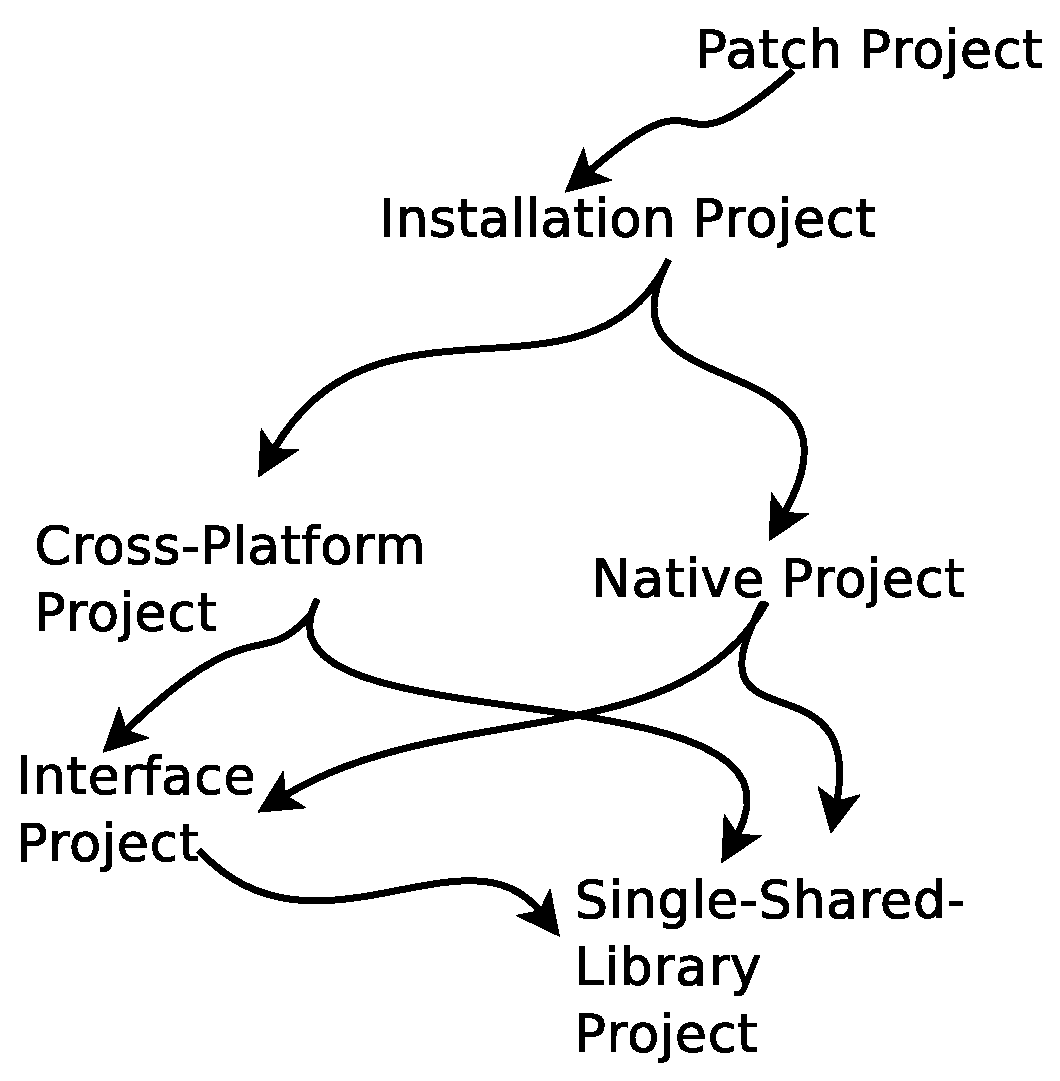
\includegraphics[width=5cm]{project-catgory-pattern-language-network.eps}
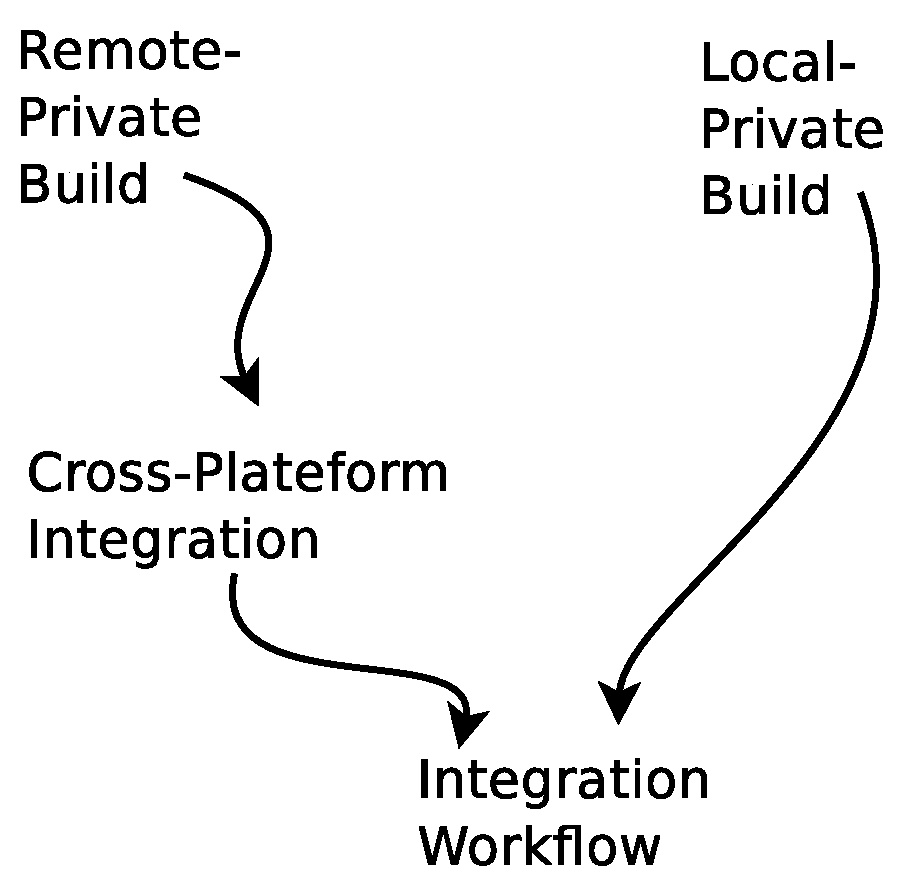
\includegraphics[width=4cm]{build-catgory-pattern-language-network.eps}

\includegraphics[width=2.5cm]{goodhabit-pattern-language.eps}
\end{frame}

\begin{frame}
\frametitle{Pattern in Action}
\begin{itemize}
\setlength{\itemindent}{1em}
\item[] 實例概述
\begin{itemize}
\item[] Web介面硬體監控軟體 ezMonitor
\item[] 與平台相關:sensor driver與利用driver讀取數據的程式碼%Linux, Windows, Driver and code need to access Driver is platform specific.%讀取硬體監控sensor數據
\item[] 與平台無關:Web 介面、控制sensor數據呈現於Web介面之模組
\end{itemize}
\item[] 與建置、佈署軟體相關樣式
\begin{itemize}
\item[] Installation Project, Single Shared Library Project, Patch Project
\end{itemize}
\item[] 與架構設計相關樣式
\begin{itemize}
\item[] Interface Project, Native Project, Cross-Platform Project
\end{itemize}
\end{itemize}
\begin{center}
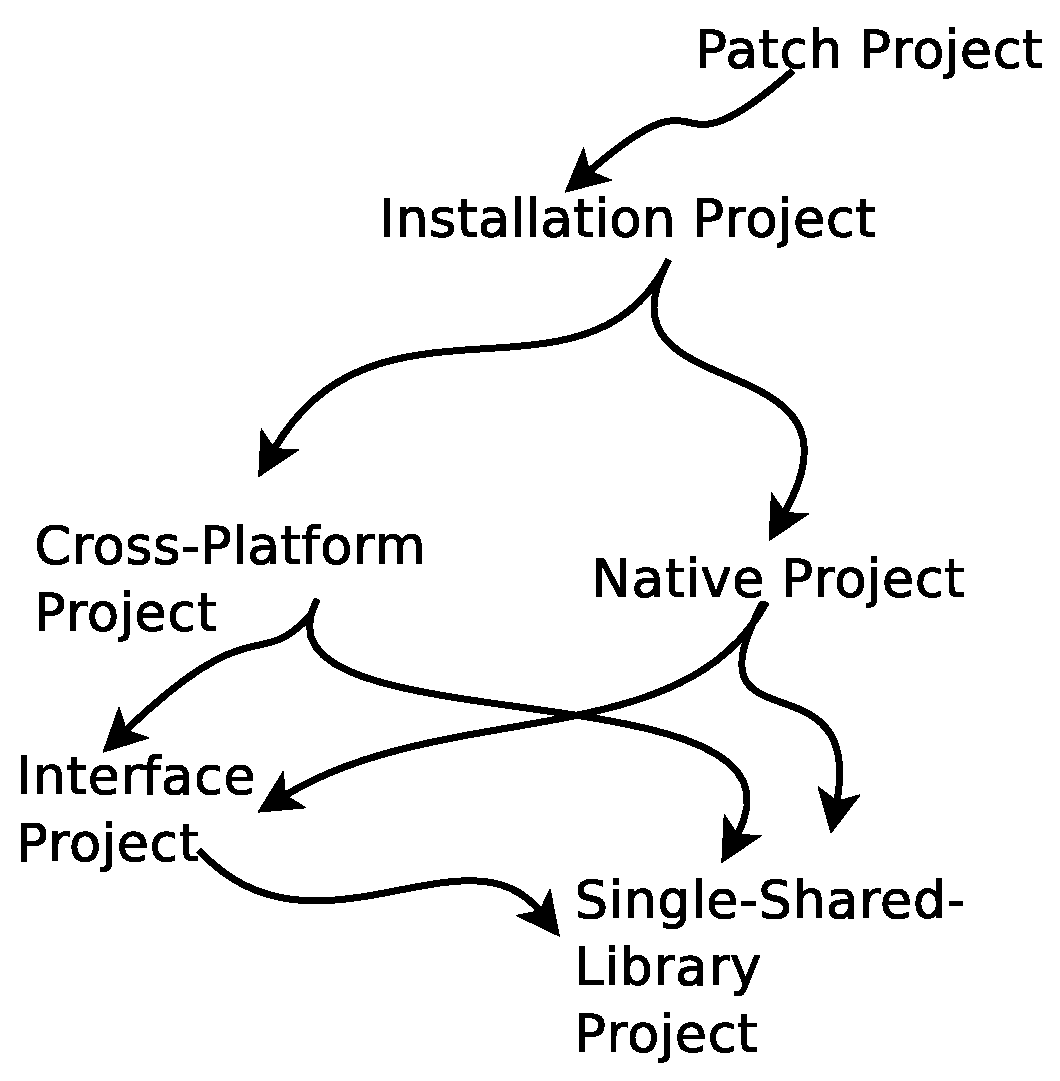
\includegraphics[width=4cm]{project-catgory-pattern-language-network.eps}
\end{center}
\end{frame}

%\begin{frame}
%\frametitle{跨平台軟體持續整合\\樣式語言 \textendash\hspace{6pt}Build 範疇樣式語言}
%\begin{center}
%\end{center}
%\end{frame}

%\begin{frame}
%\frametitle{跨平台軟體持續整合\\樣式語言 \textendash\hspace{6pt}Good Habit 範疇樣式語言}
%\begin{enumerate}
%\item 僅提出Single Responsible Person樣式
%\item 需加入與Single Responsible Person樣式有關之樣式
%\item 形成網絡關係進而形成樣式語言
%\end{enumerate}
%\end{frame}

%\begin{frame}
%\frametitle{於Portland Pattern Repository發表的\\持續整合樣式}
%\begin{enumerate}
%\item 以非正規形式表達
%\item 分享經驗與相關知識
%\item 與其他軟體開發知識領域相關
%\begin{enumerate}
%\item Software Configuration Management
%\begin{enumerate}
%\item Use One Code Line
%\item Commit Early and Often
%\item Reduce Size of Check In
%\end{enumerate}
%\item Extreme Programming
%\begin{enumerate}
%\item Collective Code Ownership
%\end{enumerate}
%\end{enumerate}
%\item 擷取其中樣式加入跨平台持續整合樣式語言
%\end{enumerate}
%\end{frame}

% \begin{frame}%---------跨平台軟體持續整合樣式語言的實例 outline page 
%\frametitle{跨平台軟體持續整合樣式語言的實例 Outline} 
%\textit{In order to discover patterns which are alive\\we must always start with observation.} \begin{flushright}Christopher Alexander, The Timeless Way of Building(1979), p.254.\end{flushright}
%\begin{enumerate}
%\item 研究方法
%\item Project 範疇樣式語言實例探討
%\item Build 範疇樣式語言實例探討
%\item Good Habit 範疇樣式語言實例探討-\hspace{3pt}Single Responsible Person樣式
%\end{enumerate}     
 %\end{frame}
 
 \begin{frame}%--------觀察實例之方法
 \frametitle{研究方法}
 \begin{itemize}
 \setlength{\itemindent}{1em}
 \item[] 軟體建置構面:概念相近之程式碼會被編譯成一可以佈署的檔案
 \item[] 檔案目錄結構構面:概念相近之程式碼會被置放於同一目錄(模組)、(專案)
 \item[] 架構設計構面:了解處於不同目錄中之程式碼如何產生關連
 \item[] 專案社群文件構面:各種討論軟體開發與持續整合相關議題之網站與書籍
 \end{itemize}
 \begin{center}
 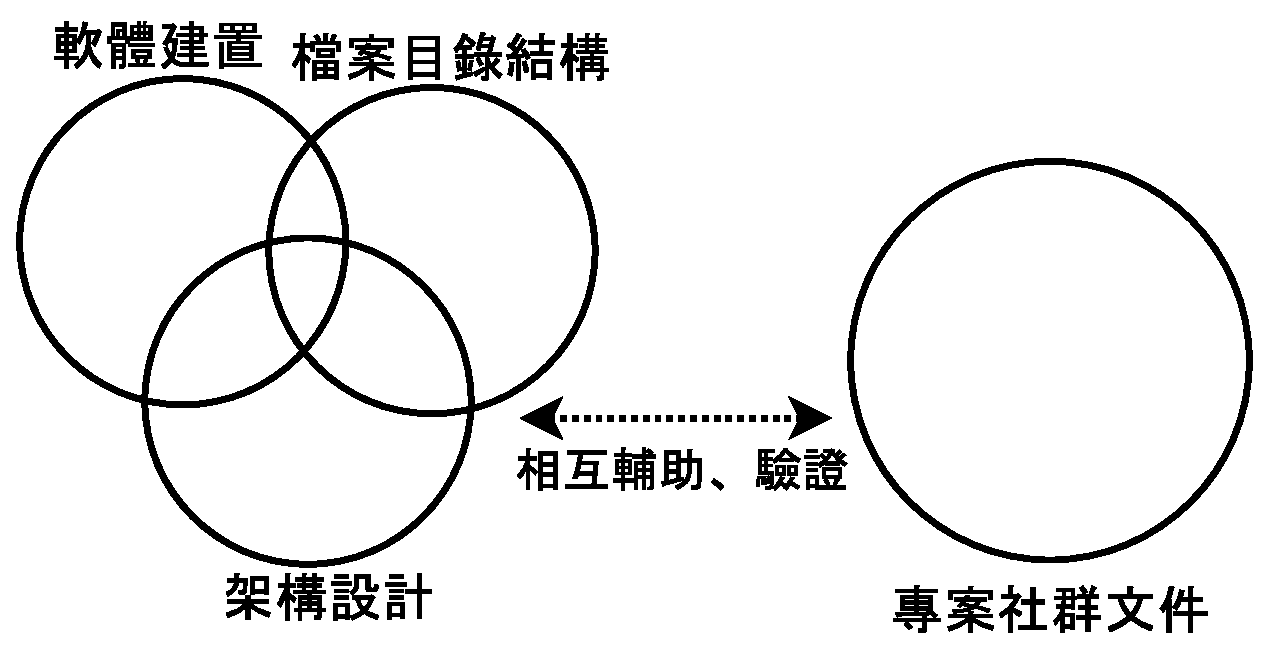
\includegraphics[width=5cm]{observation_view.eps}
 \end{center}
 \end{frame}

\begin{frame}
\frametitle{研究方法討論}
\begin{table}[!htbp]
\fontsize{9pt}{10pt}\selectfont
	\setlength{\abovecaptionskip}{0pt}
	\setlength{\belowcaptionskip}{10pt}
	\begin{center}
	%\caption{Chromium專案的子專案與子目錄}\label{subprojectfolderview}
\begin{tabular}[width=\textwidth]{|c|c|c|c|c|}
\hline
樣式\構面&軟體建置&檔案目錄結構&架構設計&專案社群文件\\
\hline
Installation Project&${\surd}$&&&${\surd}$\\
\hline
Single Shared Library Project&&&&\\
\hline
Interface Project&${\surd}$&${\surd}$&${\surd}$&${\surd}$\\
\hline
Cross-Platform Project&${\surd}$&${\surd}$&${\surd}$&${\surd}$\\
\hline
Native Project&${\surd}$&${\surd}$&${\surd}$&${\surd}$\\
\hline
Patch Project&&&&\\
\hline
\end{tabular}
\end{center}
\end{table}
\end{frame}

%\begin{frame}%---------介紹Chromium專案
%\frametitle{Chromium 專案介紹}
%\begin{enumerate}
%\item Google贊助之瀏覽器軟體專案
%\item 佔有10\%市佔率
%\item 開放原始碼、跨平台軟體
%\item Windows, Linux, Mac OS X.
%\item 以C, C++, Objective-C實作
%\begin{enumerate}
%\item 於Mac OS X,各平台通用的程式碼以C,C++實作,與UI相關的程式碼以Objective-C實作。
%\end{enumerate}
%\end{enumerate}
%\end{frame}

%\begin{frame}%--------介紹SWT專案
%\frametitle{SWT 專案介紹}
%\begin{enumerate}
%\item Java GUI框架
%\item JNI 技術
%\end{enumerate}
%\end{frame}

%\begin{frame}%--------Chromium Project Case Study
%\frametitle{Project 範疇樣式語言實例探討\hspace{3pt}-\hspace{3pt}Chromium}
%\begin{enumerate}
%\item 於Mac OS X平台觀察
%\item 從軟體建置構面出發
%\item 並以檔案目錄結構、架構設計與專案社群文件構面輔助說明。
%\end{enumerate}
%\end{frame}

%\begin{frame}
%\frametitle{軟體建置構面}%-------條列專案中子專案與子目錄
%\begin{table}[!htbp]
%	\setlength{\abovecaptionskip}{0pt}
%	\setlength{\belowcaptionskip}{10pt}
%	\begin{center}
	%\caption{Chromium專案的子專案與子目錄}\label{subprojectfolderview}
%\begin{tabular}[width=\textwidth]{|c|c|c|}
%\hline
%專案名稱&&\\
%\hline
%chrome&&\\
%\hline
%&\textit{子目錄}&\\
%\hline
%&\textit{Source}&\textit{Intermediates}\\
%\hline
%&\textit{Frameworks}&\textit{Product}\\
%\hline
%&\textit{Projects}&\textit{Build}\\
%\hline
%&\textit{Projects}所涵蓋的子專案&\\
%\hline
%&content&base\\
%\hline
%&WebCore&webkit\\
%\hline
%&Webkit&skia\\
%\hline
%&...&...\\
%\hline
%\end{tabular}
%\end{center}
%\end{table}
%\end{frame}

\begin{frame}%------Project範疇樣式語言
\frametitle{探討Project範疇樣式語言已知案例-\\\hspace{4pt}以Chromium \dag 專案為實例}
%\begin{center}
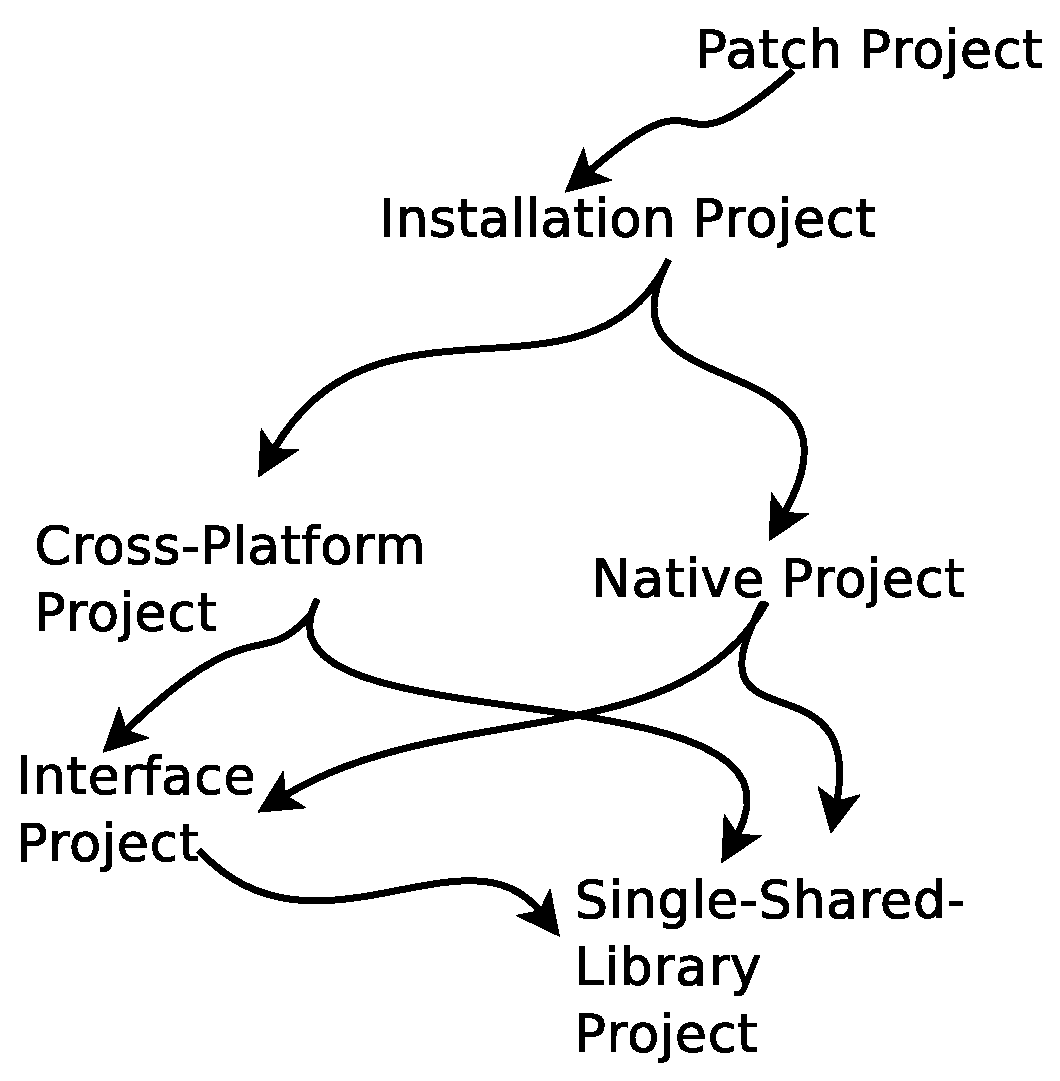
\includegraphics[width=4.5cm]{project-catgory-pattern-language-network.eps}
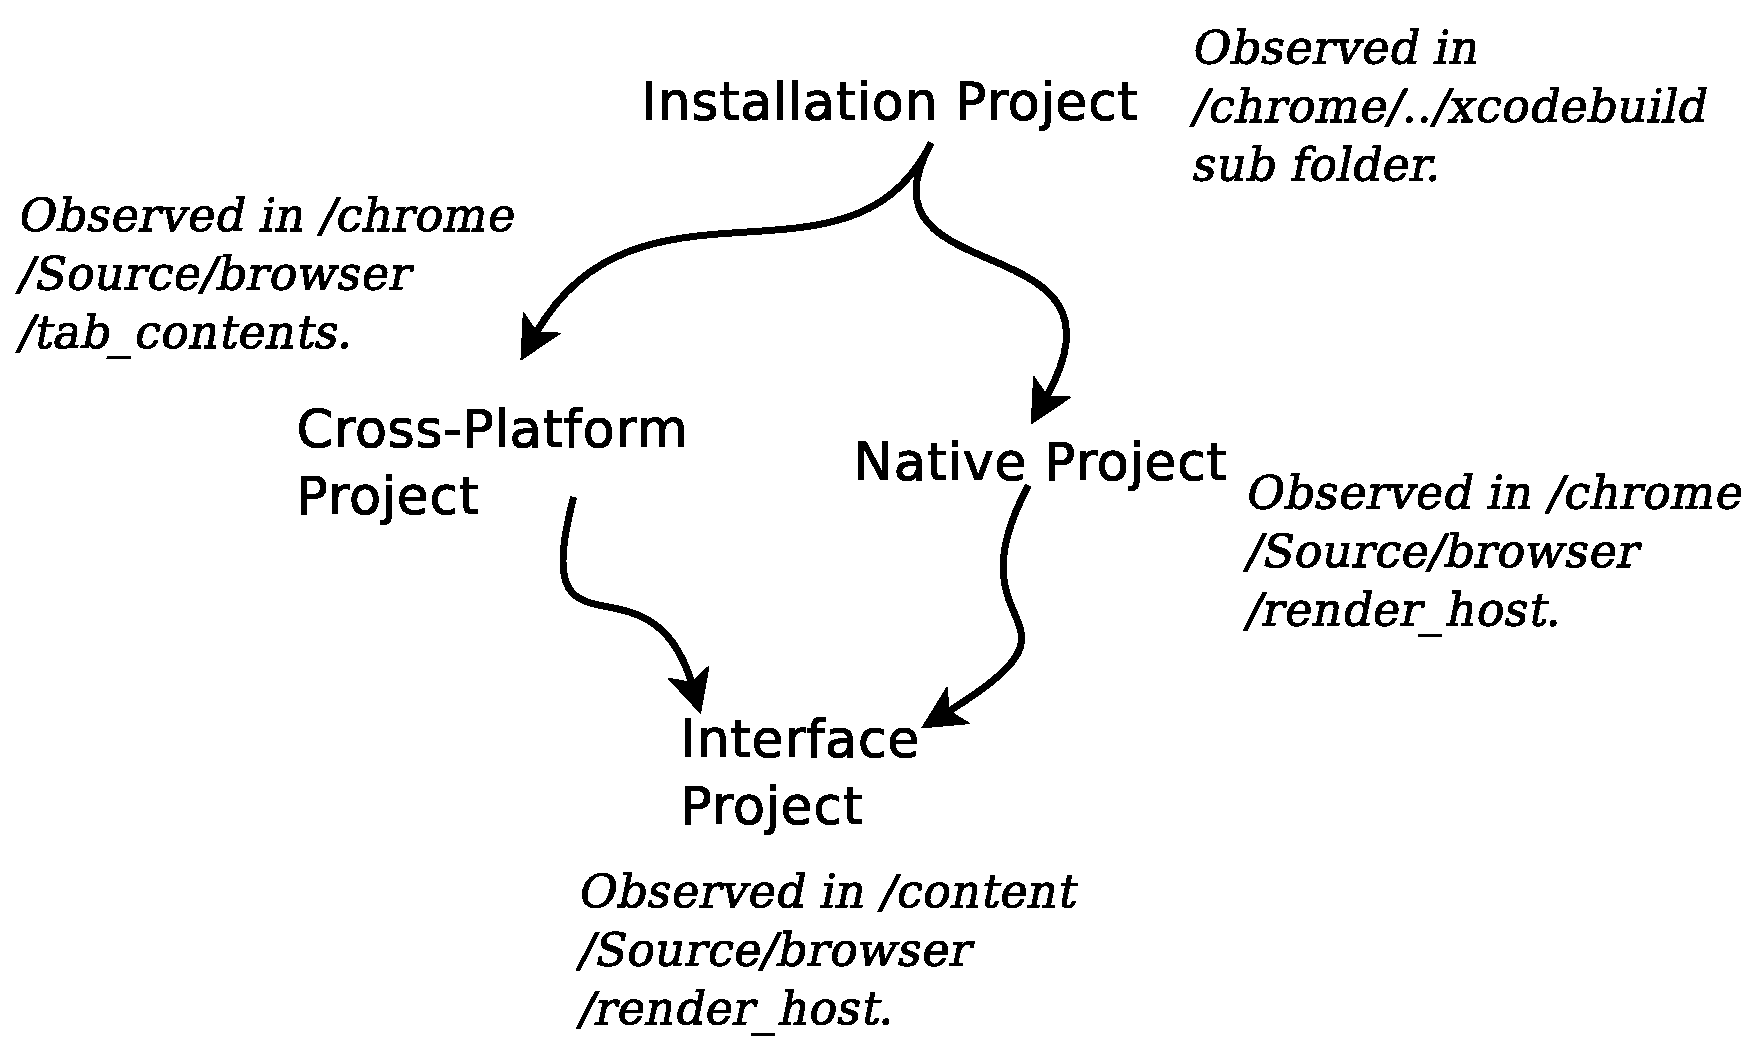
\includegraphics[width=7.5cm]{chromium-project-category-analysis-view.eps}
%\end{center}
\begin{itemize}
\fontsize{8pt}{8pt}\selectfont
\item[\dag] \url{http://www.chromium.org/Home}
\end{itemize}
\end{frame}

\begin{frame}
\frametitle{軟體建置構面}
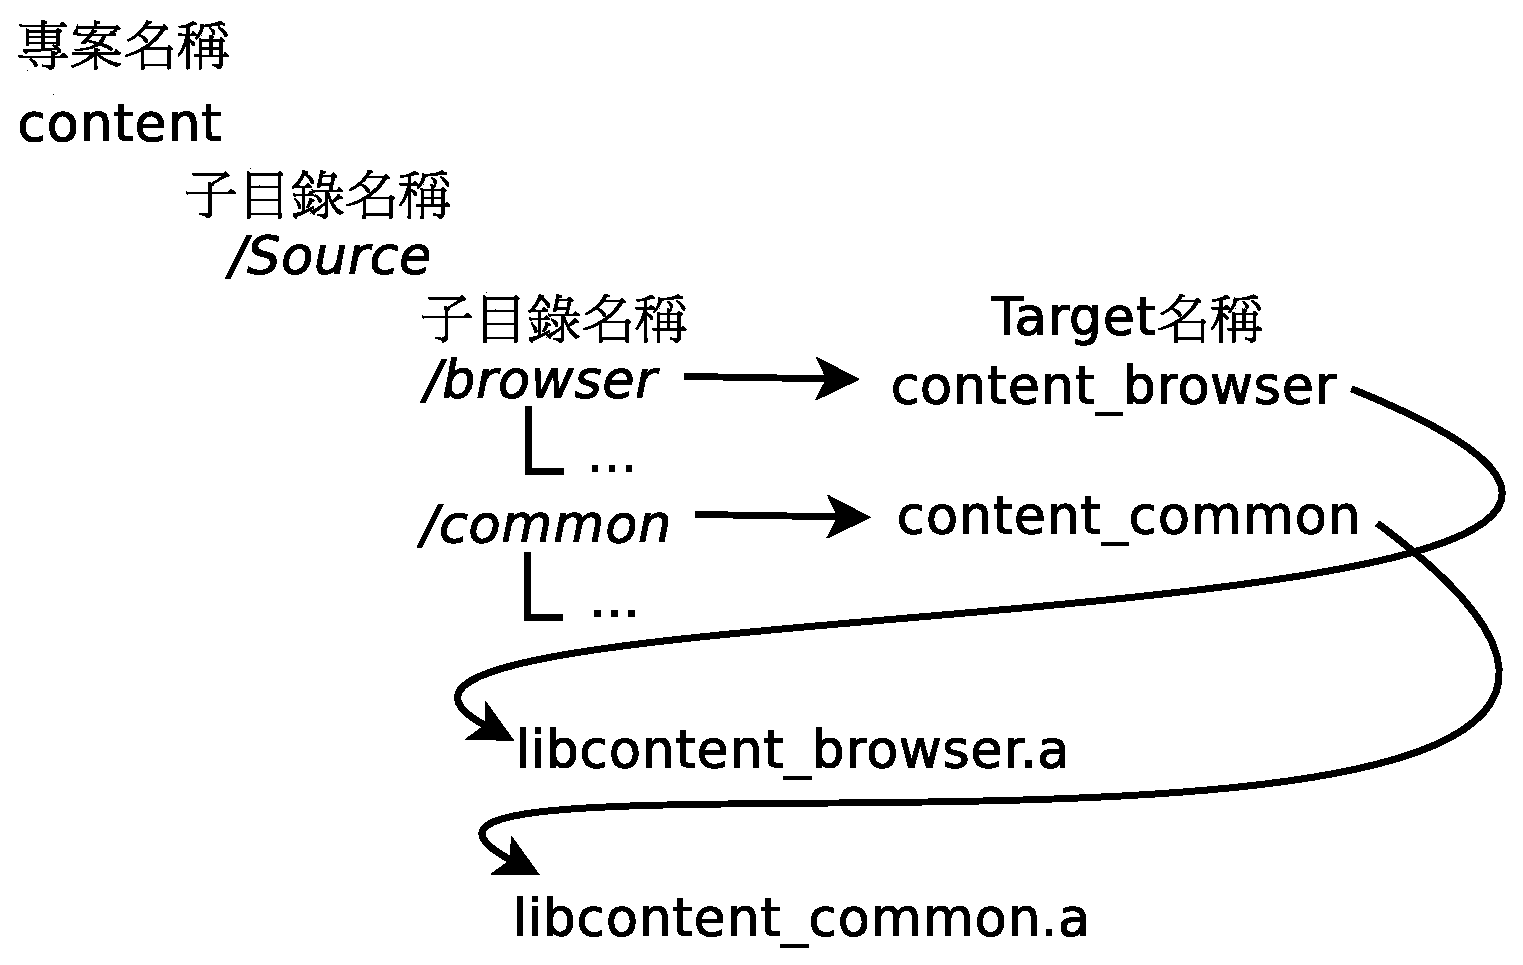
\includegraphics[width=6cm]{deploymentview.eps}
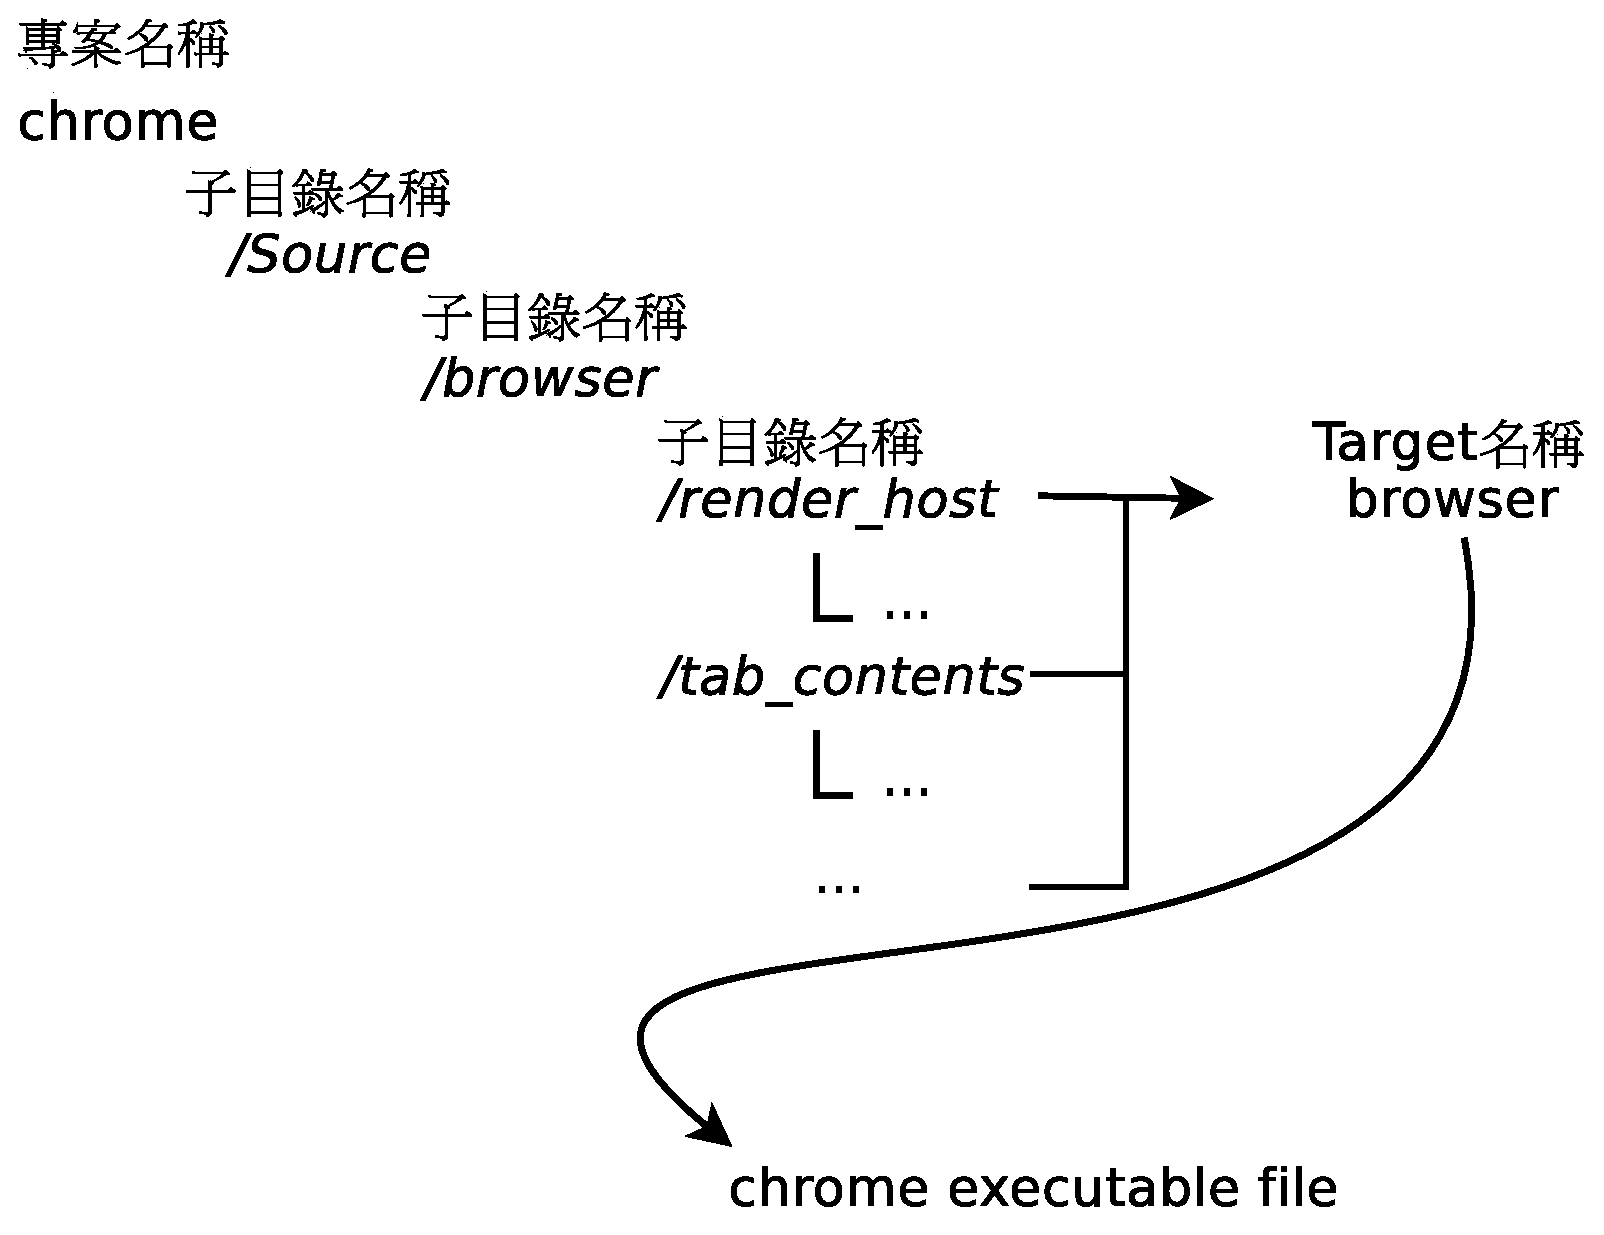
\includegraphics[width=6cm]{deploymentview-chrome.eps}
\end{frame}

\begin{frame}%------設計構面
\frametitle{架構設計構面}
\begin{center}
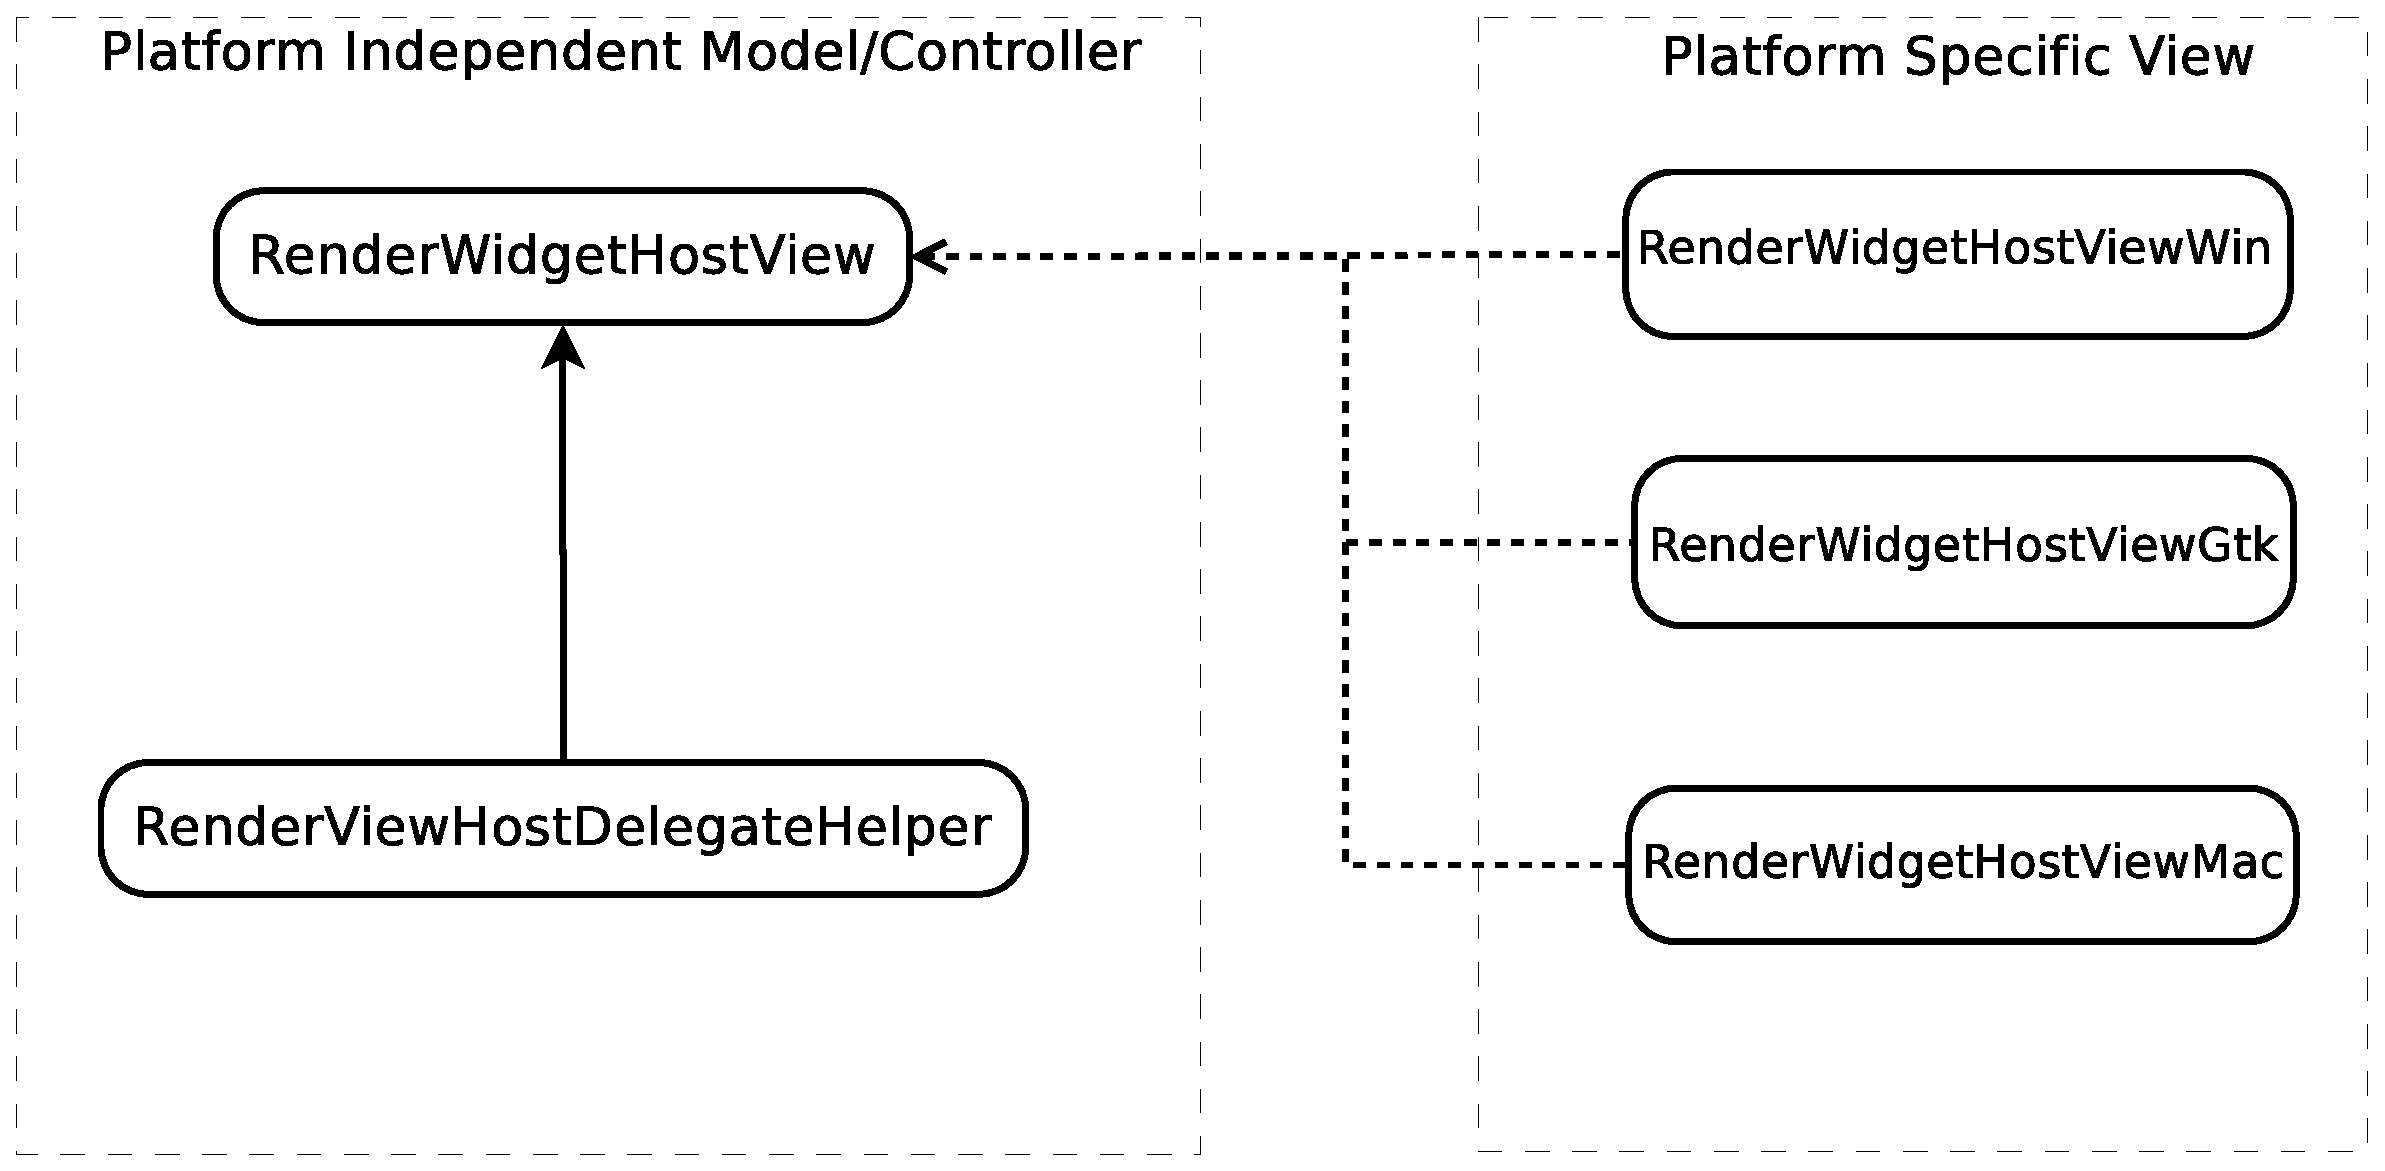
\includegraphics[width=10cm]{chromium-mvc.eps}
\end{center}
\end{frame}

%\begin{frame}
%\frametitle{軟體建置構面}
%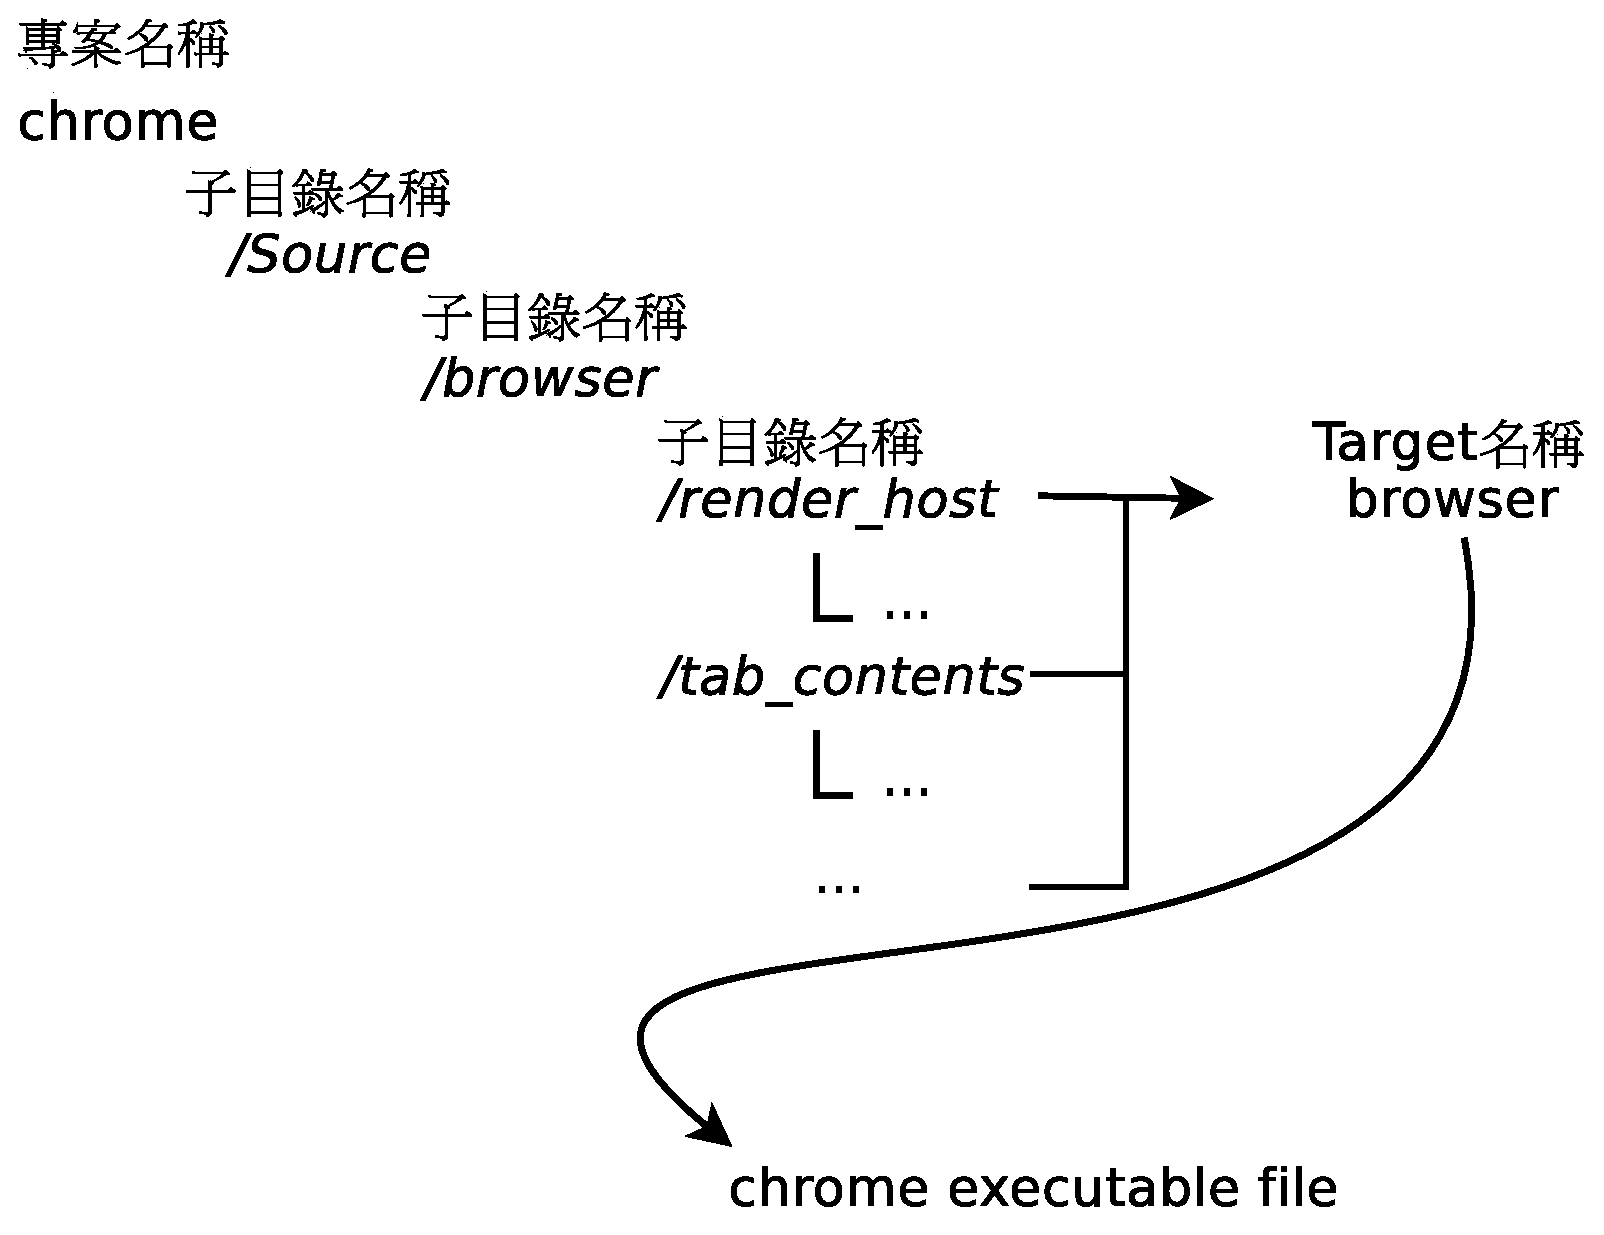
\includegraphics[width=10cm]{deploymentview-chrome.eps}
%\end{frame}

\begin{frame}[fragile,t]%------設計構面-介面定義
\frametitle{架構設計構面-\\介面定義、與平台無關之程式碼呼叫介面}
\begin{table}[h]
\begin{center}
\begin{minipage}{72mm}
\linespread{0.8}
\fontsize{8pt}{6pt}\selectfont
\begin{Verbatim}[numbers=left,framesep=1mm,numbersep=1pt] 
	節錄自render_widget_host_view.h
	    Class RenderWidgetHostView{
	    public:
	        virtual ~RenderWidgetHostView();
	        ...
	        static RenderWidgetHostView* Create
	            ViewForWidget(RenderWidgetHost
	            View* widget);
	          ...
	  }
\end{Verbatim}
\end{minipage}
\end{center}
\end{table}
\begin{table}[h]
\begin{center}
\begin{minipage}{72mm}
\linespread{0.8}
\fontsize{8pt}{6pt}\selectfont
\begin{Verbatim}[numbers=left,framesep=1mm,numbersep=1pt]
節錄自render_view_host_delegate_helper.cc
    RenderWidgetHostView*
      RenderViewHostDelegateViewHelper::
       CreateNewWidget(int route_id, 
       WebKit::WebPopupType popup_type, 
       RenderProcessHost* process) {
         RenderWidgetHost* widget_host =
         new RenderWidgetHost(process, route_id);
         RenderWidgetHostView* widget_view =
         RenderWidgetHostView::
         CreateViewForWidget(widget_host);
         ...
   }
\end{Verbatim}
\end{minipage}
\end{center}
\end{table}
\end{frame}

\begin{frame}[fragile,t]%------設計構面-平台相關實作
\frametitle{架構設計構面-與平台相關之實作}
\begin{table}[h]
\begin{center}
\begin{minipage}{72mm}
\linespread{0.8}
\fontsize{8pt}{6pt}\selectfont
\begin{Verbatim}[numbers=left,framesep=1mm,numbersep=1pt] 
	節錄自render_widget_host_view_win.cc 
	    RenderWidgetHostView* RenderWidgetHostView
	    ::CreateViewForWidget(RenderWidgetHostView*
	    widget){
	        return new RenderWidgetHostViewWin(widget);
	    }
\end{Verbatim}
\end{minipage}
\end{center}
\end{table}
\begin{table}[h]
\begin{center}
\begin{minipage}{72mm}
\linespread{0.8}
\fontsize{8pt}{6pt}\selectfont
\begin{Verbatim}[numbers=left,framesep=1mm,numbersep=1pt] 
	節錄自render_widget_host_view_gtk.cc 
	    RenderWidgetHostView* RenderWidgetHostView
	    ::CreateViewForWidget(RenderWidgetHostView*
	    widget){
	        return new RenderWidgetHostViewGtk(widget);
	    }
\end{Verbatim}
\end{minipage}
\end{center}
\end{table}
\begin{table}[h]
\begin{center}
\begin{minipage}{72mm}
\linespread{0.8}
\fontsize{8pt}{6pt}\selectfont
\begin{Verbatim}[numbers=left,framesep=1mm,numbersep=1pt] 
	節錄自render_widget_host_view_mac.cc 
	    RenderWidgetHostView* RenderWidgetHostView
	    ::CreateViewForWidget(RenderWidgetHostView*
	    widget){
	        return new RenderWidgetHostViewMac(widget);
	    }
\end{Verbatim}
\end{minipage}
\end{center}
\end{table}
\end{frame}

\begin{frame}%-------檔案目錄結構構面
\frametitle{檔案目錄結構構面}
\begin{figure}

	\psscalebox{0.54}{\psset{%linecolor= bisque,%
			nodesep=2pt,%,
			 treemode=D,%
			 levelsep=*1.5cm}
\pstree{\Tr{chrome.xcodeproject}}
			 {\pstree{\Tr{chrome}}{
			    {\pstree{\Tr{\textit{Source}}}
			 	{\pstree{\Tr{\textit{browser}}}
					{\pstree{\Tr{\textit{tab\_contents}}}
					  {\Tr{\underline{render\_view\_host\_delegate\_helper.cc}}
					  }
					  \pstree{\Tr{\textit{render\_host}}}
					  {\Tr{\underline{render\_widget\_host\_view\_*}}
					  }
					  \Tr{...}
					}
				   \Tr{...} 
				}
				
			   }
			 	\pstree{\Tr{content}}
				   {\pstree{\Tr{\textit{Source}}}
					{\pstree{\Tr{\textit{browser}}}
			 			{\pstree{\Tr{\textit{render\_host}}}
					  	{\Tr{\underline{render\_widget\_host\_view.h}}
					  	%{\Tr{render\_widget\_host\_view\_gtk.cc}}
					  	%{\Tr{render\_widget\_host\_view\_mac.mm}}
					  	}
					  	\Tr{...}
					}
				 	{\Tr{...}}
					}
				          \Tr{...}	
				  }
				  
			 \Tr{...}
			 }
			}
			}
		
\begin{center}
%\caption{專案結構與目錄結構 - Chromium,其中子目錄以斜體字體標示,原始碼檔案以底線標示,子專案以正常字體標示。}
\label{fig-folderstructure}
\end{center}
\end{figure}
\end{frame}

%\begin{frame}[fragile]%------設計構面-Linux平台實作
%\frametitle{設計構面-Linux平台實作}
%\begin{figure}
%\linespread{0.8}
%\begin{Verbatim}[numbers=left,framesep=1mm,numbersep=1pt] 
%	節錄自render_widget_host_view_gtk.cc 
%	    RenderWidgetHostView* RenderWidgetHostView
%	    ::CreateViewForWidget(RenderWidgetHostView*
%	    widget){
%	        return new 
%	        RenderWidgetHostViewGtk(widget);
%	    }
%\end{Verbatim}
%\linespread{1}
%\end{figure}
%\end{frame}

%\begin{frame}[fragile]%------設計構面-Mac平台實作
%\frametitle{設計構面-Mac平台實作}
%\begin{figure}
%\linespread{0.8}
%\begin{Verbatim}[numbers=left,framesep=1mm,numbersep=1pt] 
%	節錄自render_widget_host_view_mac.cc 
%	    RenderWidgetHostView* RenderWidgetHostView
%	    ::CreateViewForWidget(RenderWidgetHostView*
%	    widget){
%	        return new
%	        RenderWidgetHostViewMac(widget);
%	    }
%\end{Verbatim}
%\linespread{1}
%\end{figure}
%\end{frame}

%\begin{frame}[fragile]
%\frametitle{與平台無關之程式碼呼叫介面}
%\begin{figure}
%\linespread{0.8}
%\begin{Verbatim}[numbers=left,framesep=1mm,numbersep=1pt]
%   節錄自render_view_host_delegate_helper.cc
%   RenderWidgetHostView*
%     RenderViewHostDelegateViewHelper::
%      CreateNewWidget(int route_id, 
%      WebKit::WebPopupType popup_type, 
%      RenderProcessHost* process) {
%         RenderWidgetHost* widget_host =
%         new RenderWidgetHost(process, route_id);
%         RenderWidgetHostView* widget_view =
%         RenderWidgetHostView::
%         CreateViewForWidget(widget_host);
%         ...
%   }
%\end{Verbatim}
%\caption{節錄程式碼 part5: 與平台無關之程式碼呼叫介面}
%\label{crossplatformcall}
%\end{figure}
%\end{frame}

%\begin{frame}
%\frametitle{SWT Case Study}
%\end{frame}

%\begin{frame}
%\frametitle{Build 範疇樣式語言實例探討}
%\begin{enumerate}
%\item 研究對象Chromium專案
%\item 研究專案社群文件
%\item 實際觀察專案持續整合系統運作與報表
%\end{enumerate}
%\end{frame}

\begin{frame}%------論文貢獻
\frametitle{結論}%\hspace{3pt}-\hspace{3pt}論文貢獻}
\begin{itemize}
\setlength{\itemindent}{1em}
\item[] 論文貢獻
\begin{itemize}
\item 提出探討跨平台軟體持續整合樣式之研究方法
\item 成功尋獲已知案例
%\item 演化樣式語言
\end{itemize}
\item[] 未來可能研究方向
\begin{itemize}
\item 持續地觀察與演化
\item 針對以不同類型程式語言撰寫的軟體探討其已知案例
%\item 以貼近持續整合之觀點深入探討
%\item 針對Chromium專案進行實驗
\end{itemize}
\end{itemize}
\end{frame}

%\begin{frame}%------未來可能研究方向
%\frametitle{結論\hspace{3pt}-\hspace{3pt}未來可能研究方向}
%\begin{enumerate}
%\item 持續地觀察與演化
%\item 針對以不同類型程式語言撰寫的軟體探討其已知案例
%\end{enumerate}
%\end{frame}


\end{document} 


